\scanpage{133}
\margin{\uline{fuseau} \unsure{avec}
\[\left\{\begin{array}{ll}
\deleted{\unsure{b}}\inserted{a}&\text{des deux rives }\inserted{\text{(= côtés des \unsure{bigones})}}\text{ du fuseau}\\
\deleted{\unsure{\rho}}\inserted{\sigma}&\text{des deux extrémités}\\
\Omega&\text{\uline{des deux} orientations du fuseau}\\
&\boxed{\Omega\simeq a\wedge\sigma}\\
\unsure{\Omega'}&\text{ens des orientations de }X\text{ en le sommet du fuseau}
\end{array}\right.\]
\[\Omega'\simeq\Omega\wedge\sigma\simeq a\]
Si on a choisi un $D\in a$, alors $a\simeq\{\pm1\}$,
$\deleted{\unsure{\Longleftrightarrow}}\quad\Omega\simeq\sigma\simeq\omega$
(ens des orientations de $D$)}
\figure{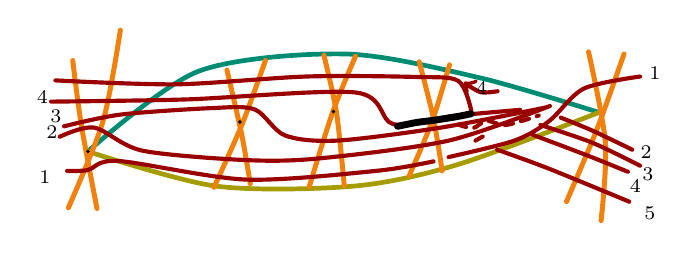
\begin{tikzpicture}[x=.55cm,y=-.55cm,line cap=round,line join=round,g/.style={olive!80!yellow,line width=1.7pt},r/.style={orange!80!brown,line width=1.8pt},w/.style={red!60!black,line width=1.5pt},b/.style={blue!60!black,line width=1.4pt},p/.style={gray!70,thin},k/.style={black,line width=1.2pt},every node/.style={font=\scriptsize}]
\draw[blue!45!green,line width=1.7pt] plot[smooth] coordinates {(3.65,5) (6.2,3.15) (9.6,2.75) (12.7,3.3) (15.45,4.1)};
\draw[olive!80!yellow,line width=1.7pt] plot[smooth] coordinates {(3.65,5) (6.6,5.8) (9.8,5.8) (12.2,5.3) (15.45,4.1)};
\draw[r] plot[smooth] coordinates {(3.3,2.9) (3.5,4.4) (3.86,6.32)};
\draw[r] plot[smooth] coordinates {(4.4,2.2) (4.0,4.3) (3.2,6.3)};
\draw[r] plot[smooth] coordinates {(6.86,3.12) (7.2,4.6) (7.4,5.75)};
\draw[r] plot[smooth] coordinates {(7.75,2.9) (7.2,4.4) (6.56,5.83)};
\draw[r] plot[smooth] coordinates {(9.1,2.78) (9.39,4.1) (9.57,5.79)};
\draw[r] plot[smooth] coordinates {(9.83,2.8) (9.3,4.1) (8.76,5.82)};
\draw[r] plot[smooth] coordinates {(11.3,2.93) (11.63,4.24) (11.83,5.45)};
\draw[r] plot[smooth] coordinates {(12.0,3.0) (11.6,4.3) (11.07,5.56)};
\draw[r] plot[smooth] coordinates {(15.21,2.7) (15.6,4.8) (15.5,6.6)};
\draw[r] plot[smooth] coordinates {(16.03,2.75) (15.4,4.5) (14.7,6.16)};
\draw[w] plot[smooth] coordinates {(2.9,3.36) (5.7,3.45) (8.7,3.27) (11.2,3.28) (12.2,3.37) (12.5,4.05)};
\draw[w] plot[smooth] coordinates {(2.8,3.85) (5.9,3.8) (9.84,3.64) (10.7,4.37) (12.1,4.18) (13.63,4.04)};
\draw[w] plot[smooth] coordinates {(3.1,4.42) (4.4,4.15) (6.5,4.0) (7.5,4.03) (8.2,4.63) (9.4,4.75) (11.8,4.45) (14.2,3.99)};
\draw[w] plot[smooth] coordinates {(3.0,4.66) (3.8,4.45) (4.9,4.98) (7.3,5.2) (9.0,5.16) (11.98,4.75) (14.32,3.95)};
\draw[w] plot[smooth] coordinates {(3.17,5.45) (3.65,5.43) (4.35,5.22) (7.3,5.65) (10.3,5.45) (11.63,5.23)};
\draw[w] plot[smooth] coordinates {(11.98,5.13) (13.5,4.75) (14.3,4.3) (15.1,3.55) (16.4,3.27)};
\draw[w] plot[smooth] coordinates {(14.57,4.22) (15.3,4.52) (16.22,4.96)};
\draw[w] plot[smooth] coordinates {(14.1,4.39) (15.3,4.8) (16.4,5.33)};
\draw[w] plot[smooth] coordinates {(13.93,4.62) (15.2,5.1) (16.12,5.47)};
\draw[w] plot[smooth] coordinates {(13.1,4.96) (14.3,5.4) (16.15,6.16)};
\draw[w,dashed] plot[smooth] coordinates {(12.2,4.38) (12.55,4.46) (12.85,4.29) (13.3,4.39) (14.06,4.17)};
\draw[w,dashed] plot[smooth] coordinates {(12.6,4.75) (12.9,4.58)};
\draw[k,line width=2.5pt] plot[smooth] coordinates {(10.8,4.42) (11.25,4.33) (11.64,4.28) (12.15,4.2) (12.5,4.13)};
\draw[w,->] plot[smooth] coordinates {(13.11,3.61) (12.71,3.63) (12.33,3.4)};
\fill[black] (3.65,5) circle (.045);
\fill[black] (7.16,4.32) circle (.045);
\fill[black] (9.32,4.08) circle (.045);
\fill[black] (11.63,4.25) circle (.045);
\node at (2.6,3.75) {$4$};
\node at (2.91,4.19) {$3$};
\node at (2.82,4.56) {$2$};
\node at (2.66,5.59) {$\unsure{1}$};
\node at (12.74,3.54) {$\unsure{4}$};
\node at (16.74,3.19) {$1$};
\node at (16.54,5.02) {$2$};
\node at (16.58,5.53) {$3$};
\node at (16.29,5.8) {$\unsure{4}$};
\node at (16.63,6.43) {$5$};
\end{tikzpicture}}
\uline{NB} ``fuseau'' $\longleftrightarrow$ p.r. \unsure{critique}, un sommet fixé dessus (``elt. de contact'')
\figure{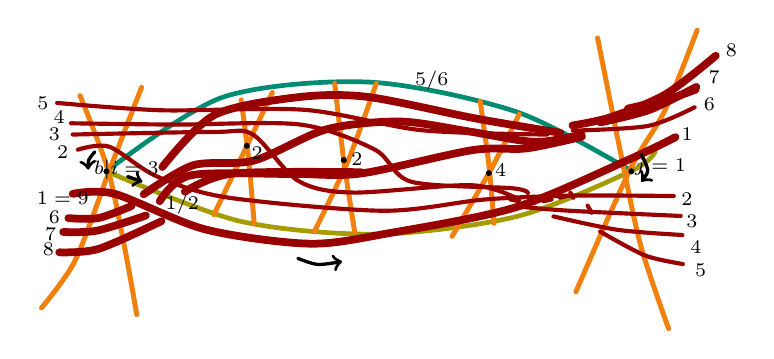
\begin{tikzpicture}[x=.55cm,y=-.55cm,line cap=round,line join=round,g/.style={olive!80!yellow,line width=1.7pt},r/.style={orange!80!brown,line width=1.8pt},w/.style={red!60!black,line width=1.5pt},b/.style={blue!60!black,line width=1.4pt},p/.style={gray!70,thin},k/.style={black,line width=1.2pt},every node/.style={font=\scriptsize}]
\draw[blue!45!green,line width=1.7pt] plot[smooth] coordinates {(5.72,10.85) (8.4,9.14) (11.8,8.79) (15.2,9.48) (17.84,10.84)};
\draw[olive!80!yellow,line width=1.7pt] plot[smooth] coordinates {(5.72,10.85) (8.8,12.0) (12.0,12.3) (15.2,11.89) (17.84,10.84) (18.39,10.4)};
\draw[r] plot[smooth] coordinates {(5.11,9.1) (5.75,10.8) (6.13,12.56) (6.42,14.16)};
\draw[r] plot[smooth] coordinates {(6.53,8.91) (5.8,10.8) (5.0,12.9) (4.22,14.0)};
\draw[r] plot[smooth] coordinates {(8.83,9.2) (9.0,10.54) (9.13,12.05)};
\draw[r] plot[smooth] coordinates {(9.55,9.03) (8.96,10.27) (8.2,11.85)};
\draw[r] plot[smooth] coordinates {(10.99,8.82) (11.2,10.6) (11.45,12.24)};
\draw[r] plot[smooth] coordinates {(11.95,8.82) (11.3,10.6) (10.52,12.24)};
\draw[r] plot[smooth] coordinates {(14.35,9.23) (14.55,10.7) (14.67,12.05)};
\draw[r] plot[smooth] coordinates {(15.25,9.53) (14.6,10.8) (13.7,12.35)};
\draw[r] plot[smooth] coordinates {(17.06,7.77) (17.6,10.46) (18.06,12.58) (18.7,14.48)};
\draw[r] plot[smooth] coordinates {(19.36,7.59) (18.61,9.45) (17.8,10.83) (16.56,13.63)};
\draw[w] plot[smooth] coordinates {(4.58,9.27) (7.0,9.44) (10.3,9.43) (13.0,9.9) (15.9,10.0)};
\draw[w] plot[smooth] coordinates {(4.9,9.74) (7.3,9.77) (10.2,9.77) (11.92,10.35) (12.76,11.09) (15.09,11.24) (15.45,11.35)};
\draw[w] plot[smooth] coordinates {(4.94,10.0) (8.2,9.94) (9.1,10.0) (10.15,11.07) (11.4,11.34) (14.15,11.17) (15.25,11.5)};
\draw[w] plot[smooth] coordinates {(5.06,10.35) (5.78,10.28) (6.87,10.96) (8.49,11.45) (12.1,11.76) (14.45,11.5) (16.5,11.41) (18.82,11.42)};
\draw[w] plot[smooth] coordinates {(15.31,11.67) (16.42,11.76) (18.98,11.88)};
\draw[w] plot[smooth] coordinates {(16.04,11.89) (17.52,12.2) (19.02,12.32)};
\draw[w] plot[smooth] coordinates {(17.12,12.24) (18.15,12.79) (19.03,12.99)};
\draw[w,line width=2.8pt] plot[smooth] coordinates {(4.94,11.37) (5.91,11.37) (8.0,12.19) (10.4,12.52) (12.23,12.28) (15.17,11.68) (17.8,10.57) (18.86,10.06)};
\draw[w,line width=2.8pt] plot[smooth] coordinates {(4.84,11.93) (5.53,11.93) (6.3,11.65)};
\draw[w,line width=2.8pt] plot[smooth] coordinates {(4.72,12.25) (5.5,12.22) (6.63,11.87)};
\draw[w,line width=2.8pt] plot[smooth] coordinates {(4.63,12.72) (5.54,12.64) (6.99,12.0)};
\draw[w,line width=2.8pt] plot[smooth] coordinates {(6.58,11.38) (7.72,10.71) (9.13,10.6) (10.8,9.88) (12.5,9.7) (14.1,9.93) (15.62,10.17) (16.69,10.0)};
\draw[w,line width=2.8pt] plot[smooth] coordinates {(6.95,11.54) (7.67,10.94) (10.01,10.91) (11.59,10.9) (14.17,10.36) (15.42,10.32) (16.7,10.05)};
\draw[w,line width=2.8pt] plot[smooth] coordinates {(7.53,11.32) (8.64,10.9) (11.6,10.87)};
\draw[w,line width=2.8pt] plot[smooth] coordinates {(7.01,10.75) (8.21,9.55) (10.12,9.14) (11.74,9.13) (14.25,9.63) (16.2,9.96)};
\draw[w,line width=2.8pt] plot[smooth] coordinates {(16.48,9.79) (17.36,9.6) (18.63,9.07) (19.79,8.18)};
\draw[w,line width=2.8pt] plot[smooth] coordinates {(17.13,9.72) (18.26,9.43) (19.34,8.9)};
\draw[w,line width=2.8pt] plot[smooth] coordinates {(17.76,9.4) (18.7,9.18) (19.33,8.96)};
\draw[w] plot[smooth] coordinates {(16.49,9.91) (18.23,9.8) (19.3,9.37)};
\draw[w,dashed] plot[smooth] coordinates {(15.05,11.5) (15.6,11.57) (16.34,11.42)};
\draw[w,dashed] plot[smooth] coordinates {(16.43,11.34) (16.5,11.46)};
\draw[w,dashed] plot[smooth] coordinates {(16.83,11.64) (17.0,11.94)};
\draw[k,->] plot[smooth] coordinates {(5.45,10.4) (5.31,10.59) (5.3,10.81)};
\draw[k,->] plot[smooth] coordinates {(6.21,10.97) (6.55,11.09)};
\draw[k,->] plot[smooth] coordinates {(10.14,12.86) (10.6,13.0) (11.16,12.93)};
\draw[k,->] plot[smooth] coordinates {(18.07,10.46) (18.22,10.83) (18.07,11.09)};
\fill[black] (5.72,10.85) circle (.07);
\fill[black] (8.96,10.26) circle (.07);
\fill[black] (11.2,10.59) circle (.07);
\fill[black] (14.55,10.89) circle (.07);
\fill[black] (17.84,10.85) circle (.07);
\node at (4.25,9.27) {$5$};
\node at (4.63,9.6) {$4$};
\node at (4.52,10.0) {$3$};
\node at (4.71,10.41) {$2$};
\node at (4.71,11.47) {$1=9$};
\node at (4.52,11.92) {$\unsure{6}$};
\node at (4.43,12.31) {$\unsure{7}$};
\node at (4.38,12.65) {$\unsure{8}$};
\node at (6.18,10.8) {$\unsure{b|i}=3$};
\node at (9.2,10.43) {$2$};
\node at (11.5,10.56) {$2$};
\node at (14.82,10.83) {$4$};
\node at (18.51,10.75) {$\unsure{j}=1$};
\node at (7.47,11.62) {$1/2$};
\node at (13.23,8.75) {$5/6$};
\node at (20.15,8.05) {$8$};
\node at (19.75,8.68) {$7$};
\node at (19.64,9.3) {$6$};
\node at (19.13,10.0) {$1$};
\node at (19.12,11.5) {$2$};
\node at (19.24,12.0) {$3$};
\node at (19.33,12.6) {$4$};
\node at (19.44,13.13) {$5$};
\end{tikzpicture}}
Ce circuit de positions relatives stables dépend de la position non-stable de départ $D$ \inserted{\unsure{avec le sommet} $s\in S_D$} (voir dessin), du choix de sa \unsure{quasiorientation} de degré $1$ i.e. de la rive correspondante $\rho$ de $D$ en $s$, et d'une \deleted{\unsure{co}}orientation $\omega$ de $D$ (pour indiquer l'ordre de succession des \deleted{\unsure{opérations}} balayages des triangles), ce qui (moyennant le choix de $\rho$) équivaut à la donnée d'une orientation $\bar\omega$ de $X$ en $s$.
\figure{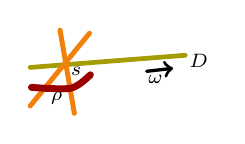
\begin{tikzpicture}[x=.55cm,y=-.55cm,line cap=round,line join=round,g/.style={olive!80!yellow,line width=1.7pt},r/.style={orange!80!brown,line width=1.8pt},w/.style={red!60!black,line width=1.5pt},b/.style={blue!60!black,line width=1.4pt},p/.style={gray!70,thin},k/.style={black,line width=1.2pt},every node/.style={font=\scriptsize}]
\draw[g] plot[smooth] coordinates {(21.2,13.92) (24.78,13.64)};
\draw[r] plot[smooth] coordinates {(21.89,13.06) (22.22,14.98)};
\draw[r] plot[smooth] coordinates {(22.57,13.13) (21.2,14.81)};
\draw[w,line width=2.5pt] plot[smooth] coordinates {(21.23,14.38) (22.14,14.4) (22.59,14.09)};
\draw[k,->] (23.89,14.01)--(24.5,13.94);
\node at (22.26,14.02) {$s$};
\node at (21.81,14.64) {$\rho$};
\node at (24.09,14.2) {$\omega$};
\node at (25.09,13.76) {$D$};
\end{tikzpicture}}
On trouve donc le circuit $D_1,D_2,{-}\ D_8,D_9=D_1$. Comment trouverait-on le circuit inverse \unsure{De} $D_1=D_9,D_8,{-}\ D_3,D_2$ ? C'est en changeant \uline{à la fois} la rive $\rho$, et l'orientation $\omega$.

Ainsi, l'opération $\sigma_2$ sur les repères de $\widetilde X$ correspond à l'opération qui \deleted{\unsure{change fixe}} \uline{fixe} $\bar\omega$ (orientation en $s$) et qui change $\omega$ (orientation de $D$, \deleted{\unsure{i.e. de}} \inserted{un} flanc du fuseau)
\figure{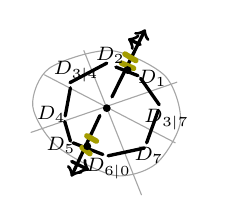
\begin{tikzpicture}[x=.55cm,y=-.55cm,line cap=round,line join=round,g/.style={olive!80!yellow,line width=1.7pt},r/.style={orange!80!brown,line width=1.8pt},w/.style={red!60!black,line width=1.5pt},b/.style={blue!60!black,line width=1.4pt},p/.style={gray!70,thin},k/.style={black,line width=1.2pt},every node/.style={font=\scriptsize}]
\draw[p] plot[smooth cycle] coordinates {(18.08,16.22) (19.34,16.8) (19.7,17.86) (19.13,18.84) (18.16,19.1) (16.85,18.43) (16.29,17.5) (16.67,16.63)};
\draw[p] (16.56,16.78)--(19.58,18.35);
\draw[p] (16.25,18.11)--(19.62,16.95);
\draw[p] (17.47,16.22)--(18.8,19.55);
\draw[k] plot[smooth] coordinates {(17.15,16.96) (18.0,16.51)};
\draw[k] plot[smooth] coordinates {(17.16,17.08) (17.04,17.73)};
\draw[k] plot[smooth] coordinates {(17.03,17.86) (17.16,18.31)};
\draw[k] plot[smooth] coordinates {(17.22,18.35) (17.91,18.62)};
\draw[k] plot[smooth] coordinates {(18.03,18.65) (18.87,18.47)};
\draw[k] plot[smooth] coordinates {(18.92,18.35) (19.19,17.6)};
\draw[k] plot[smooth] coordinates {(19.21,17.47) (18.78,16.86)};
\draw[k] plot[smooth] coordinates {(18.72,16.8) (18.21,16.6)};
\draw[k,->] plot[smooth] coordinates {(18.12,17.29) (18.89,15.73)};
\draw[k,->] plot[smooth] coordinates {(17.84,17.72) (17.18,19.13)};
\draw[g,line width=2pt] plot[smooth] coordinates {(18.34,16.51) (18.62,16.63)};
\draw[g,line width=2pt] plot[smooth] coordinates {(18.42,16.3) (18.67,16.45)};
\draw[g,line width=2pt] plot[smooth] coordinates {(17.54,18.19) (17.76,18.31)};
\draw[g,line width=2pt] plot[smooth] coordinates {(17.43,18.46) (17.61,18.6)};
\draw[k,->] plot[smooth] coordinates {(18.77,16.08) (18.49,15.95)};
\draw[k,->] plot[smooth] coordinates {(17.19,18.78) (17.59,18.98)};
\fill[black] (18.0,17.55) circle (.09);
\fill[black] (18.48,16.67) circle (.09);
\fill[black] (17.55,18.43) circle (.09);
\node at (18.08,16.33) {$D_2$};
\node at (19.05,16.87) {$D_1$};
\node at (19.38,17.82) {$D_{\unsure{3|7}}$};
\node at (18.97,18.64) {$D_{\unsure{7}}$};
\node at (18.04,18.94) {$D_{\unsure{6|0}}$};
\node at (16.94,18.41) {$D_5$};
\node at (16.72,17.69) {$D_{\unsure{4}}$};
\node at (17.29,16.71) {$D_{\unsure{3|4}}$};
\end{tikzpicture}}
Donner $(D,\bar\omega,\omega)$ revient \unsure{---} $\unsure{=}$ \unsure{que de} donner le fuseau qu'il définit, avec \deleted{\unsure{un} $\unsure{\omega}$} une \unsure{orientation} du fuseau $\Longleftrightarrow$ une orientation $\bar\omega$ de $X$ en \unsure{le|son} sommet, et un sommet (extrémité) du fuseau i.e. une \unsure{des|de} \unsure{Composantes}.
\margin{\mspage{132}}
